\section{Modelo Entidad Relación}

%TODO: agregar una introducción pequenia?
\begin{figure}[H]
  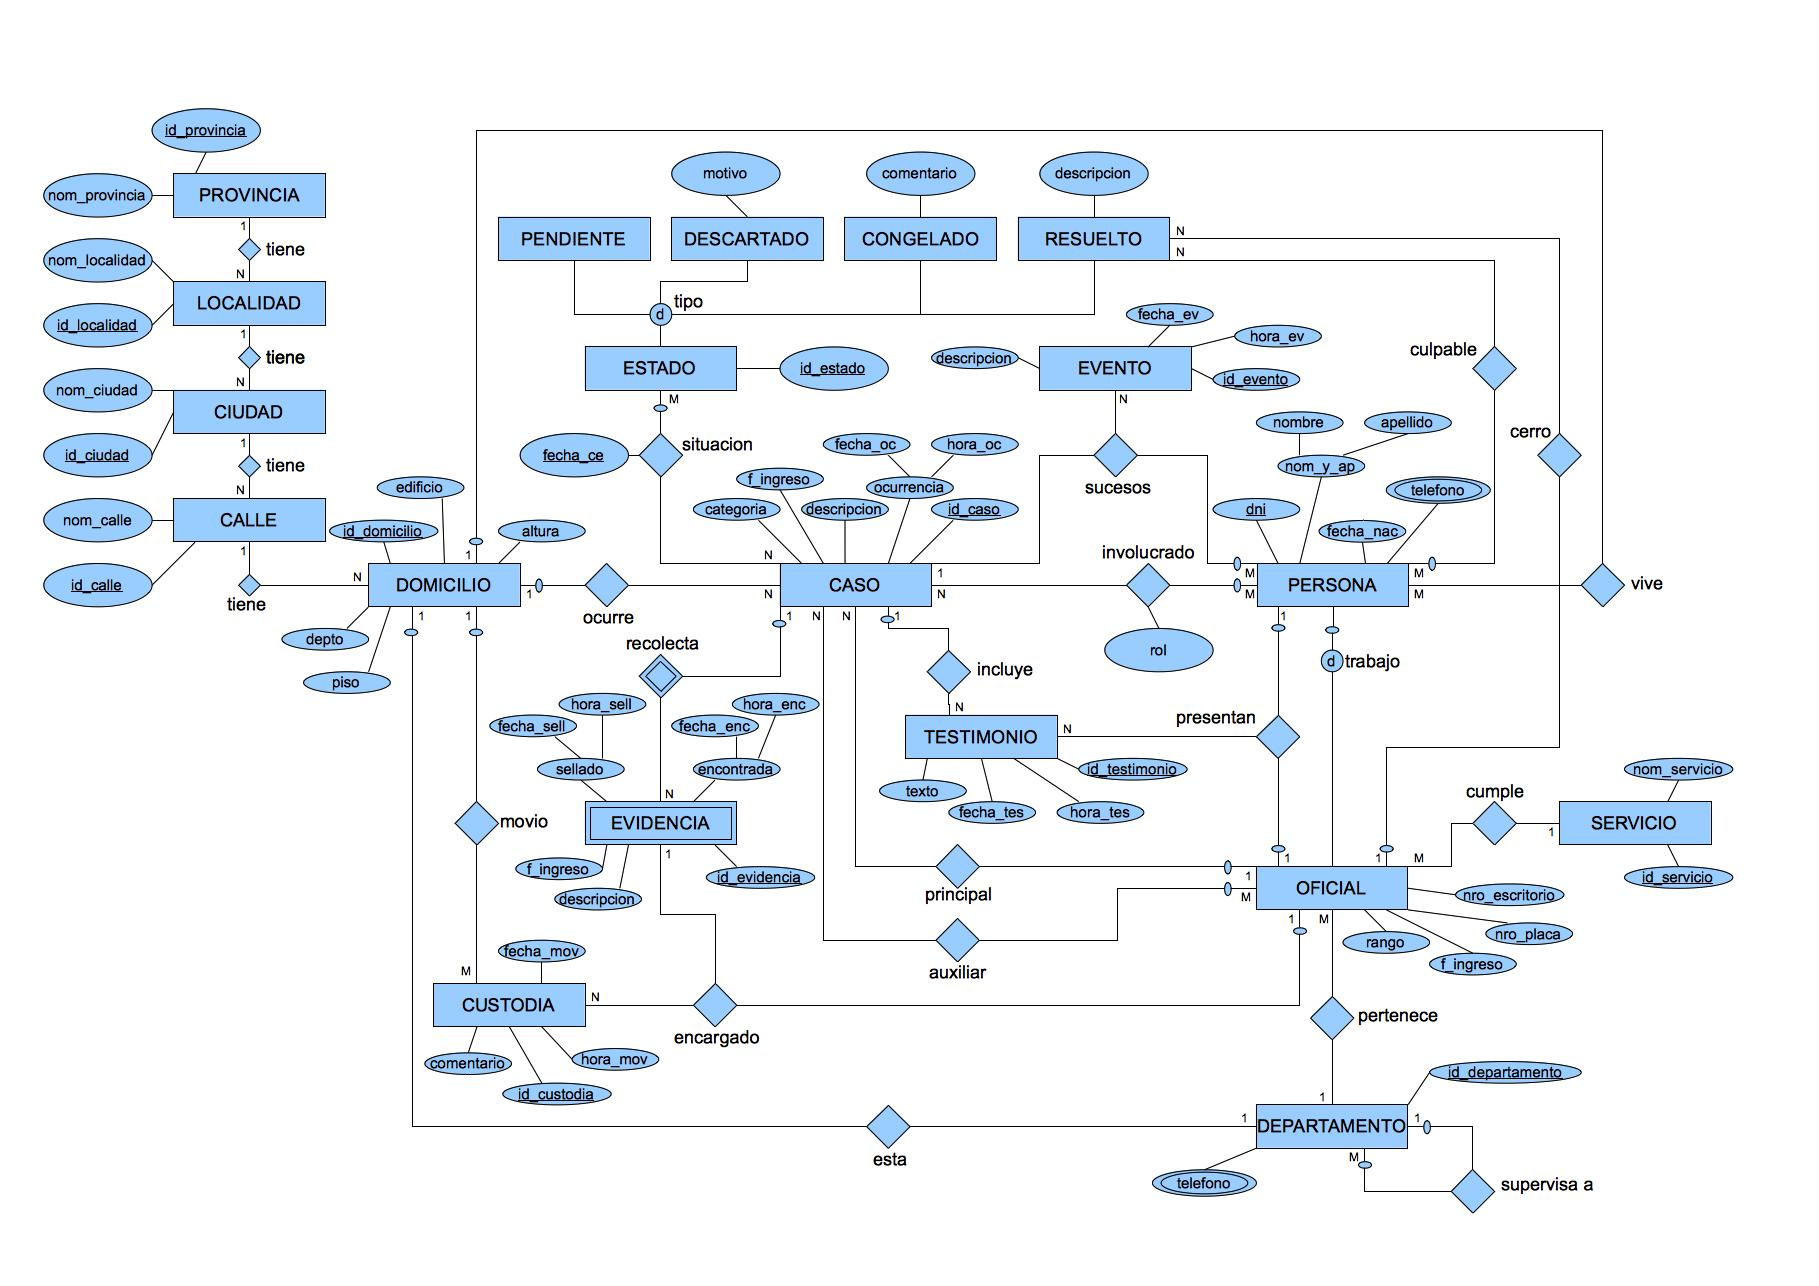
\includegraphics[angle=90, width=\linewidth]{figuras/DER.jpg}
  \caption{Modelo Entidad Relación.}
  \label{fig:MER}
\end{figure}

\subsection{Restricciones adicionales}

\begin{itemize}
\item La fecha de ingreso de un caso debe ser posterior a la fecha de ocurrencia.

\item La fecha de ingreso de la evidencia debe ser posterior a la fecha de recolección.

\item La fecha de recolección de evidencia debe ser posterior a la fecha de ingreso del caso correspondiente.

\item La fecha de ocurrencia de un evento debe ser anterior a la fecha de ingreso del caso correspondiente.

\item Si se tiene una tupla $\langle c,o\rangle$ en principal, entonces no puede estar la misma tupla en auxiliar o viceversa.

\item Dada una tupla $\langle p,r \rangle$ en culpable, $\langle c,e \rangle$ en situación y $e.id\_estado$ $=$ $r.id\_estado$, entonces tiene que existir una tupla $\langle c,p,rol \rangle$ en involucrado.

\item Dada una tupla $\langle c,e,p \rangle$ en sucesos debe existir la tupla $\langle c,r,p \rangle$ en involucrado.

\item Dada una tupla $\langle c,r,p \rangle$ en involucrado, si p además es un oficial, dicho oficial no puede estar relacionado con el caso c a través de principal o auxiliar.

\item Dada una tupla $\langle t,o,p \rangle$ en presentan, $o.dni = p.dni$

\item Dada la tupla $\langle o,r \rangle$ en cerro, debe existir una tupla $\langle c,o \rangle$ en principal o en auxiliar tal que $c.id\_caso$ $\neq$ $r.id\_caso$.
\end{itemize}
